%--------------------
% Packages
% -------------------
\documentclass[11pt,a4paper]{article}


\usepackage[pdftex]{graphicx} % Required for including pictures
\usepackage[pdftex,linkcolor=black,pdfborder={0 0 0}]{hyperref} % Format links for pdf
\usepackage{calc} % To reset the counter in the document after title page

\frenchspacing % No double spacing between sentences
\linespread{1.2} % Set linespace
\usepackage[a4paper, lmargin=0.1666\paperwidth, rmargin=0.1666\paperwidth, tmargin=0.1111\paperheight, bmargin=0.1111\paperheight]{geometry} %margins

\usepackage[protrusion=true,expansion=true]{microtype} % Improves typography, load after fontpackage is selected


%-----------------------
% Set pdf information and add title, fill in the fields
%-----------------------
\hypersetup{
pdfsubject = {Software Product Engineering},
pdftitle = {SCEEM Space - Requirements},
pdfauthor = {Jason Park, Sungijn Kang, William Nafack, Calum West}
}

%-----------------------
% Begin document
%-----------------------
\begin{document}

\begin{titlepage}
   \vspace*{\stretch{1.0}}
   \begin{center}
      \Large\textbf{SCEEM Space - Requirements}\\
      \large\textit{Jason Park, Sungijn Kang, William Nafack, Calum West}
   \end{center}
   \vspace*{\stretch{2.0}}
\end{titlepage}

\section{Requirements}
\subsection{Identified user stakeholders for SCEEM Space:}
\begin{itemize}
    \item \textit{Staff members} of ‘The School of Computer Science, Electrical and Electronic Engineering and Engineering Maths’. These staff members are admins that have access to the SCEEM Space application and can make changes, update information, add/remove people.
\end{itemize}

\subsection{User stakeholder stories:}
These are some different 'user stories'. They are things that the user (staff members) want to be able to do when they are using the product:
\begin{itemize}
        \item Quick and easy way to add/remove spaces as the school moves/expands  into different buildings
        \item Quick and easy way to add/remove desks as more spaces become available to the school in different buildings
        \item Quick and easy way to add/remove persons as people become members of the university, or leave the university
        \item Manage (add/remove) waiting list effectively as desk space is limited. Check if there is any desk space that is about to become available for reallocation.
        \item Manage sensitive information for academics and PhD students (usernames)
        \item Need to keep track of how many offices and desk are allocated to different research groups
        \item Be able to keep track of the total number of offices/desks, see how many are free and how many are occupied/allocated to a persons
    \end{itemize}

\subsection{Identified stakeholders for SCEEM Space:}
\begin{itemize}
    \item \textit{Academics} don’t have direct access to the database and other persons information contained within the database. They will not be able to see where other people are located office/desk wise. They are stakeholders as they are affected by the information input into the system by the staff members.
    \item \textit{PhD students} don’t have direct access to the database and other persons information contained within the database. They will not be able to see where other people are located office/desk wise. They are stakeholders as they are affected by the information input into the system by the staff members.
    \item \textit{University students} are not directly affected by the system but are still stakeholders. This system is used to assign spaces desks/offices to academics and PhD students, and since university students often need to go to lecturers offices, the students are indirectly affected by where academics and PhD students are placed by the system. If an academic were to request to move office and this was accommodated by the system, the a university student would now have to go to a different place to speak to this academic.
\end{itemize}

\subsection{Flow steps for user stakeholder (staff member) stories:}
\begin{itemize}
  \item Add space:
    \begin{itemize}
      \item Navigate to application login page
      \item Login to application using provided admin login details
      \item Navigate to 'Spaces' tab
      \item Click on 'Add Space' button
      \item Enter details of space (name)
    \end{itemize}
  \item Remove space:
    \begin{itemize}
      \item Navigate to application login page
      \item Login to application using provided admin login details
      \item Navigate to ‘Spaces’ tab
      \item Click on remove space button
      \item Select space to be removed
      \item Confirm space to be removed
    \end{itemize}
  \item Add desk:
    \begin{itemize}
      \item Navigate to application login page
      \item Login to application using provided admin login details
      \item Navigate to ‘Spaces’ tab
      \item Click on space in which the desk will be added to
      \item Click on ‘Add Desk’ button
      \item Enter details of desk e.g Room, Desk status, Desk number
    \end{itemize}
  \item Remove desk:
    \begin{itemize}
      \item Navigate to application login page
      \item Login to application using provided admin login details
      \item Navigate to ‘Spaces’ tab
      \item Click on ‘space’ in which the desk will be removed from
      \item Click on ‘Remove Desk’ button
      \item Select desk to remove from ‘space’
      \item Confirm removal of desk
    \end{itemize}
  \item Add persons:
    \begin{itemize}
      \item Navigate to application login page
      \item Login to application using provided admin login details
      \item Navigate to ‘Persons’ tab
      \item Click on ‘Add Persons’ button
      \item Enter details of ‘person’ e.g Name, Email, Group, Desk occupied etc.
    \end{itemize}
  \item Remove persons:
    \begin{itemize}
      \item Navigate to application login page
      \item Login to application using provided admin login details
      \item Navigate to ‘Persons’ tab
      \item Search for ‘person’ using search bar
      \item Click on ‘Remove Persons’ button
      \item Confirm removal of ‘person’
    \end{itemize}
  \item Manage waiting list:
    \begin{itemize}
      \item Navigate to application login page
      \item Login to application using provided admin login details
      \item Navigate to ‘Waiting List’ tab (Then it will show up faculties)
      \item Click on 'faculty'
      \item Find who is waiting for an empty desk/office
      \item Add the person who is waiting
      \item Remove the person who is waiting.
    \end{itemize}
  \item Manage sensitive information:
    \begin{itemize}
      \item Navigate to application login page
      \item Login to application using provided admin login details
      \item Navigate to ‘Persons’ tab
      \item Search for ‘person’ using search bar
      \item Click on ‘Personal Information’
    \end{itemize}
  \item Access number of occupied desks/offices by group:
    \begin{itemize}
      \item Navigate to application login page
      \item Login to application using provided admin login details
      \item Navigate to ‘Groups’ tab
      \item Click on ‘groupname’ to bring up information about group
      \item Number of desks occupied by group included in information
    \end{itemize}
  \item Access total number of occupied desks/offices:
    \begin{itemize}
      \item Navigate to application login page
      \item Login to application using provided admin login details
      \item Navigate to ‘Spaces’ tab
      \item Information about the total number of offices/desks displayed at the top of page
    \end{itemize}
\end{itemize}

\subsection{Alternative flows:}
\begin{itemize}
  \item Manage waiting list:
    \begin{itemize}
      \item Navigate to application login page
      \item Login to application using provided academic/PhD-student login details
      \item Navigate to ‘Waiting List’ tab
      \item Click on ‘facultyname’
      \item Remove their name from waiting list
    \end{itemize}
  \item Access number of occupied desks/offices by group:
    \begin{itemize}
        \item Navigate to application login page
        \item Login to application using provided admin login details
        \item Navigate to 'Spaces' tab
        \item Filter by Spaces only occupied by specific group
        \item Count number of desks/offices occupied from filtered results
    \end{itemize}
\end{itemize}

\subsection{Exceptional flows:}
\textit{Exceptional} flow steps are shown in italics.
\begin{itemize}
  \item Add space:
    \begin{itemize}
       \item Navigate to application login page
       \item Login to application using provided admin login details
       \item \textit{Navigate to incorrect tab}
       \item Navigate to 'Spaces' tab
       \item \textit{Click on 'Remove Space' button}
       \item Click on 'Add Space' button
       \item \textit{Enter incorrect details for space}
       \item Remove details and enter new details for space
    \end{itemize}
\end{itemize}

\subsection{High-level Use-case Diagram}
This diagram depicts a high-level relationship between use cases, actors and the system.

\begin{figure}[!h]
    \centering
    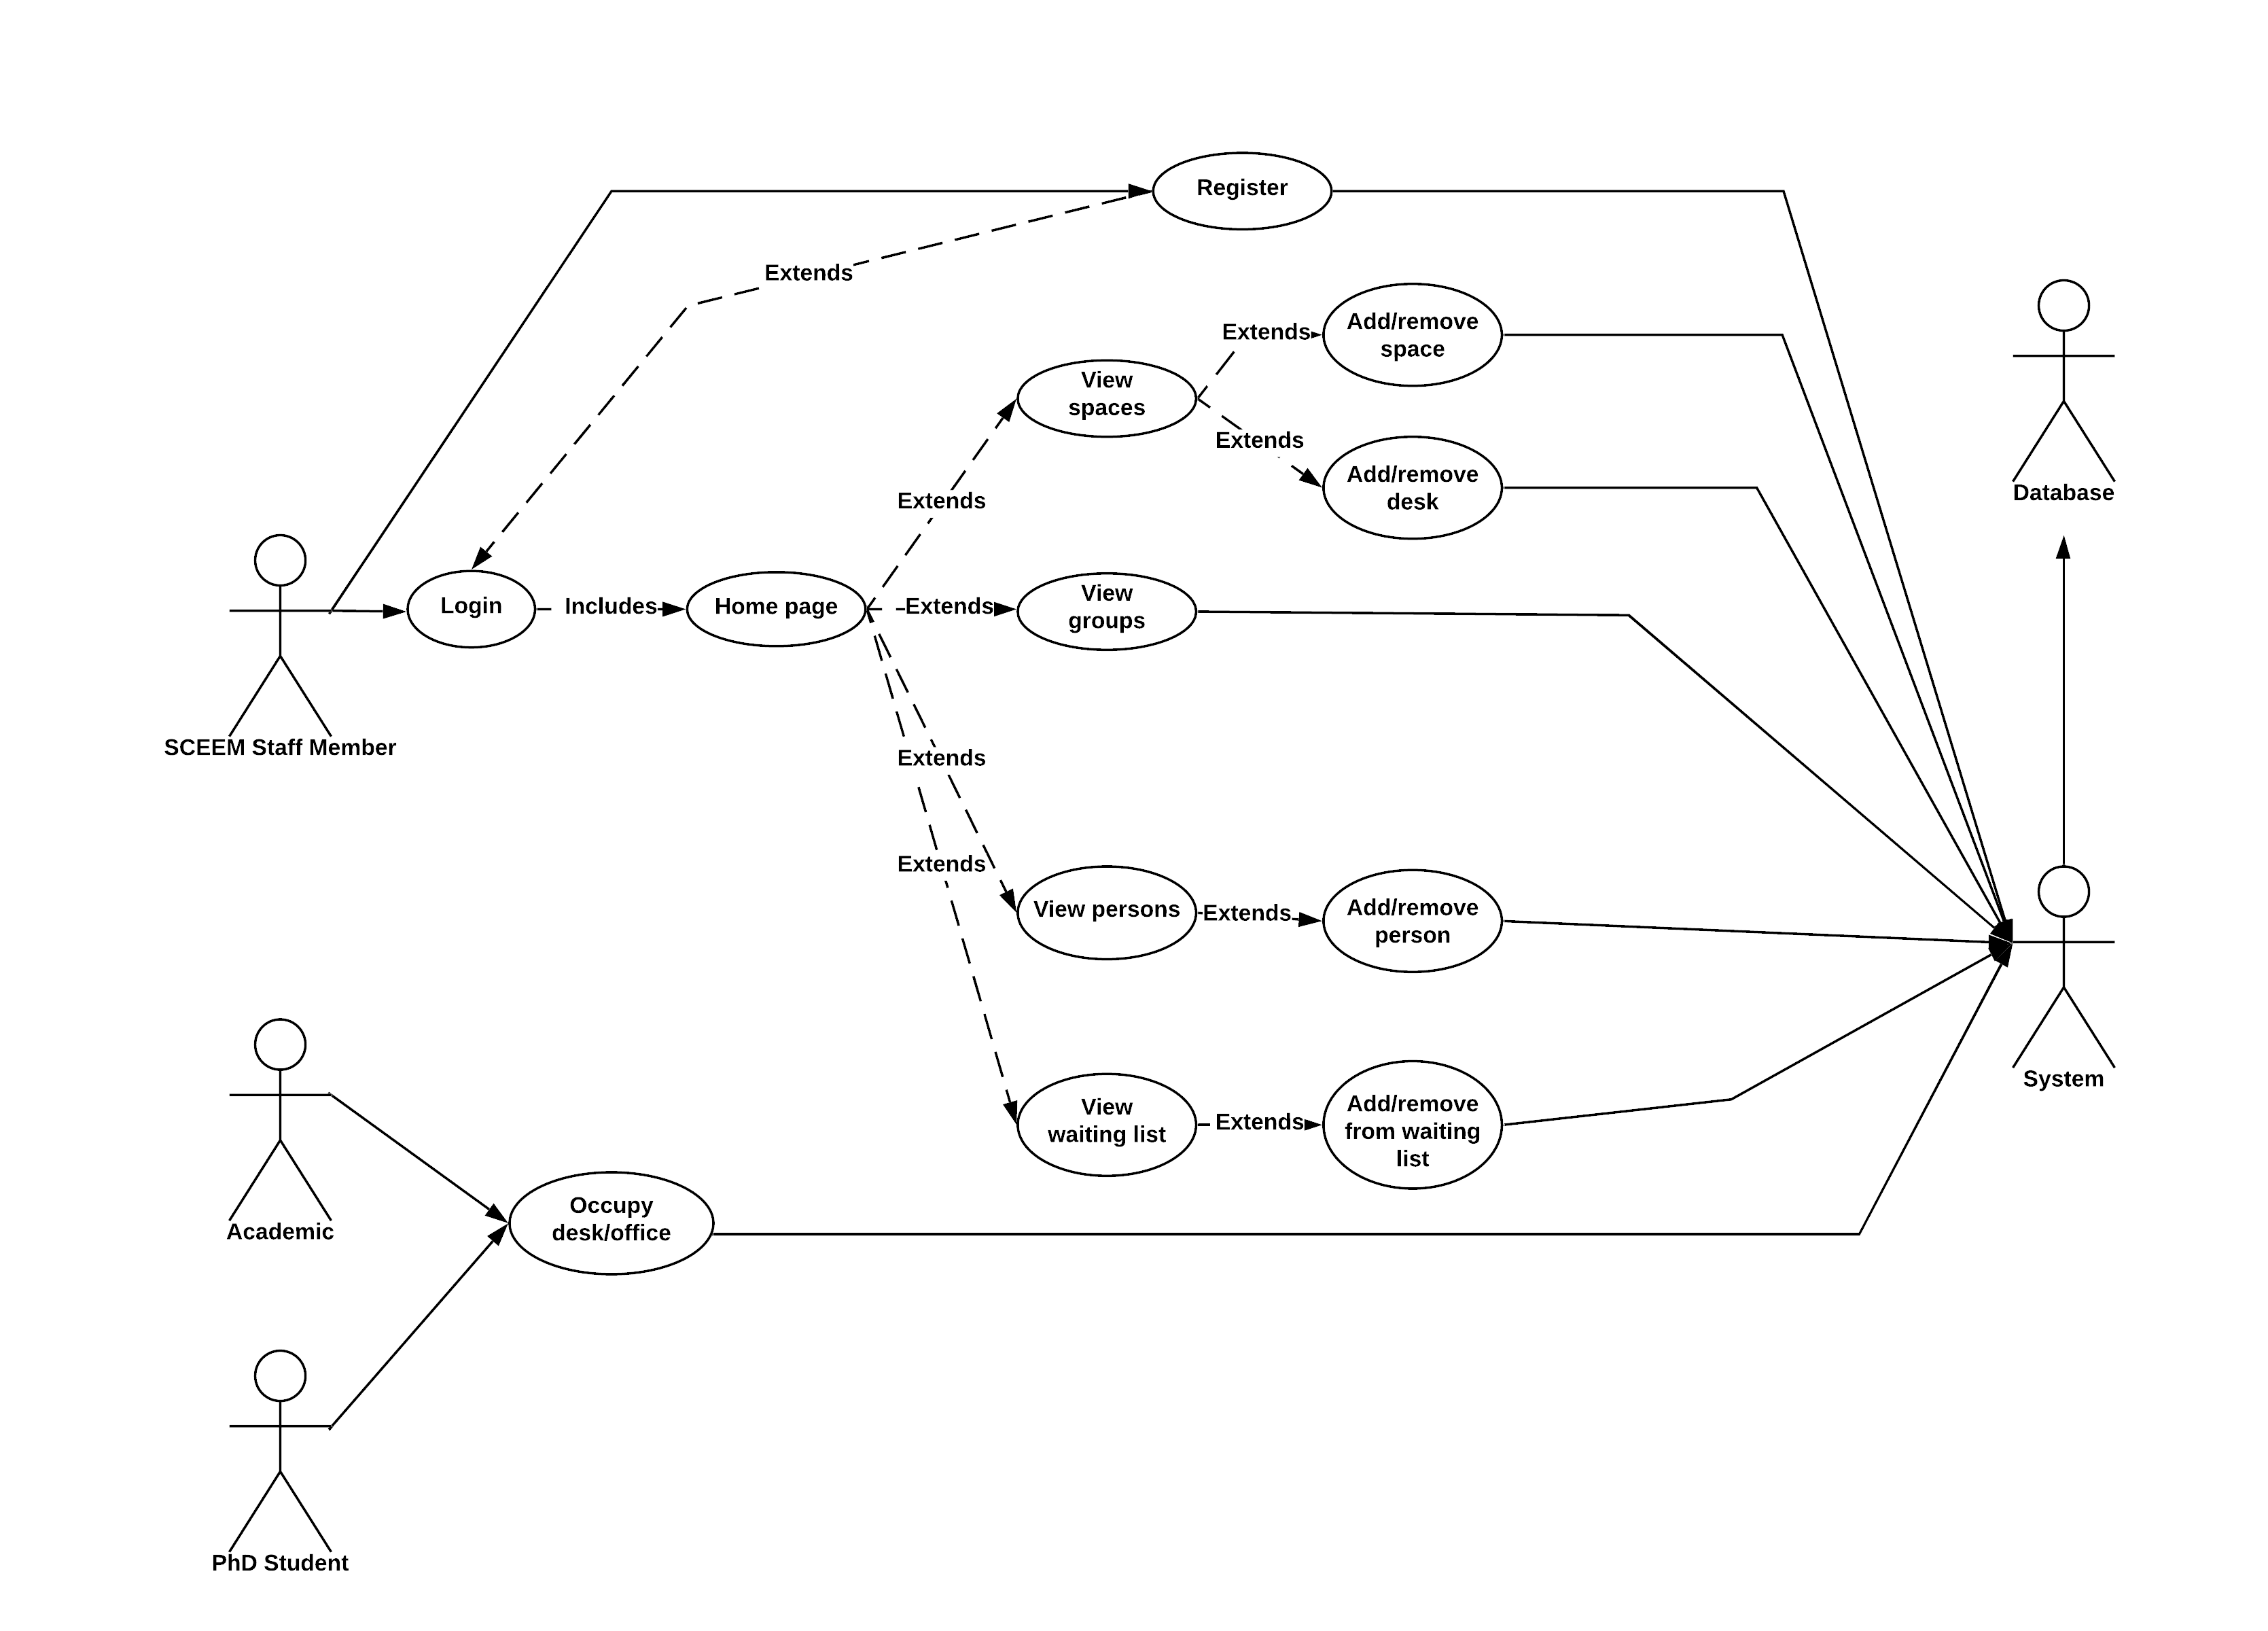
\includegraphics[width=\linewidth]{use_case.png}
    \caption{High-level Use-case diagram}
    \label{fig:basic_2}
\end{figure}

\end{document}
